\documentclass[11pt, a4paper]{article}

% Pacchetti base per lingua e codifica
\usepackage[utf8]{inputenc}
\usepackage[italian]{babel}

% Pacchetti per la matematica e la fisica
\usepackage{amsmath, amssymb, amsfonts}
\usepackage{cancel} % Utile per sbarrare i termini che si annullano

% Pacchetti per la grafica e l'impaginazione
\usepackage{graphicx}
\usepackage{geometry}
\geometry{top=2.5cm, bottom=2.5cm, left=2.5cm, right=2.5cm}
\usepackage{booktabs}
\usepackage{multirow}
\usepackage{sectsty}
\usepackage{float}
\usepackage{xcolor}
\allsectionsfont{\underline}
\setcounter{secnumdepth}{0}

\begin{document}
\tableofcontents

\newpage
\section{Interazione Radiazione Materia} %

Finora abbiamo considerato l'atomo isolato. In queste condizioni, la funzione d'onda completa (spazio-temporale) è uno \textbf{Stato Stazionario}: %
\begin{equation}
    \Psi_{nlm}(r, \theta, \varphi, t) = u_{nlm}(r, \theta, \varphi) e^{-i\frac{E_n}{\hbar}t} %
\end{equation}

\noindent
Per uno stato stazionario, l'energia è perfettamente definita ($E = E_n \Rightarrow \sigma_E = \Delta E = 0$) e, soprattutto, la densità di probabilità $|\Psi|^2$ \textbf{non dipende dal tempo}. %

\noindent
Anche se il sistema si trova in una \textbf{sovrapposizione di stati stazionari}: %
\begin{equation}
    \Psi(r,t) = \sum_{n,l,m} c_{nlm} u_{nlm} e^{-i\frac{E_n}{\hbar}t} %
\end{equation}
La probabilità di misurare una certa energia $E_n$ è data da $\mathbb{P}(E = E_n) = \sum_{l,m} |c_{nlm}|^2$. %

\textit{Esempio:} %
\begin{equation*}
    \Psi = \sqrt{\frac{3}{5}} u_{100} e^{-i\frac{E_1}{\hbar}t} + \frac{1}{\sqrt{5}} u_{200} e^{-i\frac{E_2}{\hbar}t} + \frac{1}{\sqrt{5}} u_{210} e^{-i\frac{E_2}{\hbar}t} %
\end{equation*}
\begin{equation*}
    \sum_{n,l,m} |c_{nlm}|^2 = \frac{3}{5} + \frac{1}{5} + \frac{1}{5} = 1 \quad \Rightarrow \quad \mathbb{P}(E = E_1) = \frac{3}{5} \quad , \quad \mathbb{P}(E = E_2) = \frac{2}{5} %
\end{equation*}
In assenza di perturbazioni esterne, i coefficienti $c_{nlm}$ \textbf{non dipendono mai dal tempo}. %

\begin{figure}[H]
    \centering
    \begin{minipage}{0.43\textwidth}
        \centering
        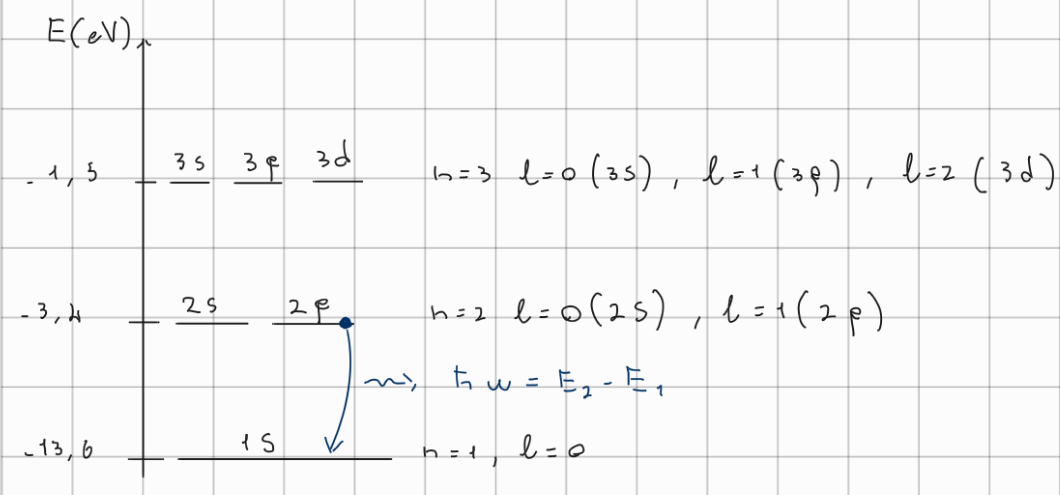
\includegraphics[width=\linewidth]{immagini/2026-04-30-18-25-33.png}
    \end{minipage}\hfill
    \begin{minipage}{0.55\textwidth}
        \textbf{Problema fondamentale:} Se gli stati sono \textit{tutti stazionari}, l'elettrone ci rimarrebbe per sempre, senza mai scendere al livello inferiore emettendo un fotone! %
        Affinché ci sia una transizione elettronica, i coefficienti della sovrapposizione devono cambiare nel tempo: $c_{nlm} = c_{nlm}(t)$ \textit{(devono dipendere dal tempo)}. %
    \end{minipage}
\end{figure}

\subsection{L'Hamiltoniana di Interazione} %

Per studiare l'interazione della materia con la radiazione Elettromagnetica (EM), consideriamo l'Hamiltoniana di una particella carica in un campo EM, dove il momento canonico diventa $\vec{p} = m\vec{v} + e\vec{A}$ (con $\vec{A}$ potenziale vettore): %
\begin{equation}
    \hat{H} = \frac{1}{2m} (\hat{\vec{p}} - e\vec{A})^2 + e\phi = \frac{1}{2m} (p^2 + e^2 A^2 - e\hat{\vec{p}}\cdot\vec{A} - e\vec{A}\cdot\hat{\vec{p}}) + V(r) %
\end{equation}

\noindent
Vediamo come si comportano gli operatori $\vec{A}$ e $\hat{\vec{p}}$. Valutiamo il loro commutatore per poter semplificare l'espressione: %
\begin{equation*}
    [\hat{p}, A(x)] = [\hat{p}, \hat{x}] \frac{\partial A}{\partial x} = -i\hbar \frac{\partial A}{\partial x} %
\end{equation*}
In 3D, questo diventa $[\hat{\vec{p}}, \vec{A}(\vec{r})] = -i\hbar (\nabla \cdot \vec{A})$. %
Ci poniamo nella \textbf{Gauge di Coulomb}, in cui si impone $\nabla \cdot \vec{A} = 0$ (divergenza nulla). %
\begin{equation*}
    [\hat{\vec{p}}, \vec{A}(\vec{r})] = -i\hbar \operatorname{div}\vec{A} = 0 \quad (\text{GAUGE DI COULOMB}) %
\end{equation*}
Poiché commutano, i due termini misti nell'Hamiltoniana sono uguali ($-e\hat{\vec{p}}\cdot\vec{A} = -e\vec{A}\cdot\hat{\vec{p}}$). L'Hamiltoniana diventa: %
\begin{equation}
    \Rightarrow \quad \hat{H} = \underbrace{ \left[ \frac{\hat{p}^2}{2m} + V(r) \right] }_{\hat{H}_0} + \underbrace{ \left[ \frac{e^2 A^2}{2m} - \frac{e}{m} \vec{A} \cdot \hat{\vec{p}} \right] }_{\hat{H}_{\text{interazione}} \text{ (termine perturbativo)} \ll \hat{H}_0} %
\end{equation}

\noindent
Essendo il campo di radiazione solitamente debole, il potenziale vettore $\vec{A}$ è piccolo. Il termine quadratico $A^2$ risulta \textbf{trascurabile} rispetto a quello lineare in $\vec{A}$. %
Quindi, l'Hamiltoniana di interazione si riduce a: %
\begin{equation}
    \Rightarrow \quad \hat{H}_{int} = - \frac{e}{m} \vec{A} \cdot \hat{\vec{p}} %
\end{equation}

\noindent
Consideriamo per $\vec{A}$ l'interpretazione classica del potenziale per un'onda piana monocromatica: %
\begin{equation*}
    \vec{A} = A_0 \hat{\varepsilon} e^{i(\vec{q}\cdot\vec{r} - \omega t)} %
\end{equation*}
(dove $\hat{\varepsilon}$ è il versore di polarizzazione e $\vec{q}$ il vettore d'onda della radiazione). %

\noindent
Sostituendo in $\hat{H}_{int}$ e separando esplicitamente la dipendenza temporale: %
\begin{equation}
    \hat{H}_{int} = - \frac{e}{m} A_0 e^{i(\vec{q}\cdot\vec{r} - \omega t)} \hat{\varepsilon} \cdot \hat{\vec{p}} = \hat{L} e^{-i\omega t} %
\end{equation}
Dove abbiamo definito l'operatore spaziale $\hat{L}$: %
\begin{equation}
    \boxed{ \hat{L} = - \frac{e}{m} A_0 e^{i(\vec{q}\cdot\vec{r})} \hat{\varepsilon} \cdot \hat{\vec{p}} } %
\end{equation}

\subsection{Evoluzione dei Coefficienti nel Tempo} %

Con l'aggiunta del termine di interazione $\hat{H}_{int}$, le autofunzioni di $\hat{H}_0$ non sono più soluzioni del problema. Le autofunzioni di $\hat{H}_0$ costituiscono comunque un insieme completo che quindi posso scrivere come combinazione lineare per la nuova $\Psi$ %:
\begin{equation}
    i\hbar \frac{\partial \Psi}{\partial t} = \hat{H} \Psi \qquad \text{con } \Psi = \sum_k c_k(t) u_k(\vec{r}) e^{-i\omega_k t} \quad , \quad \omega_k = \frac{E_k}{\hbar} %
\end{equation}

\noindent
All'istante iniziale $t=0$, supponiamo che il sistema si trovi in un singolo autostato iniziale $i$: %
\begin{equation*}
    \Rightarrow \quad \Psi(\vec{r}, t=0) = u_i(\vec{r}) \quad \text{con energia } E = E_i %
\end{equation*}

L'Hamiltoniana totale è la somma della parte imperturbata e della perturbazione: %
\begin{equation*}
    \hat{H} = \hat{H}_0 + \hat{H}_{int} \qquad \text{dove } \hat{H}_{int} = \hat{L} e^{-i\omega t} %
\end{equation*}

Sostituiamo la sommatoria nell'equazione di Schrödinger dipendente dal tempo: %
\begin{align*}
    i\hbar \frac{\partial}{\partial t} &= \hat{H} \Psi \quad \Rightarrow \quad i\hbar \left[ \sum_k \dot{c}_k u_k(\vec{r}) e^{-i\omega_k t} + \sum_k c_k \frac{\partial \Psi}{\partial t} (u_k e^{-i\omega_k t} )\right] = \\ %
    &= (\hat{H}_0 + \hat{H}_{int}) \sum_k c_k u_k(\vec{r}) e^{-i\omega_k t} %
\end{align*}

\noindent
Posso \textbf{semplificare i primi due addendi} da ambo le parti perché $i\hbar \frac{\partial \Psi}{\partial t} = \hat{H}_0 \Psi$ per la parte imperturbata %.

\begin{equation*}
    i\hbar \frac{\partial}{\partial t} (u_k(\vec{r}) e^{-i\omega_k t}) \leftrightarrow \hat{H}_0 (u_k(\vec{r}) e^{-i\omega_k t}) %
\end{equation*}

Rimaniamo con l'equazione che lega le derivate dei coefficienti al termine di interazione: %
\begin{equation}
    \Rightarrow \quad i\hbar \sum_k \dot{c}_k u_k e^{-i\omega_k t} = \sum_k \hat{H}_{int} c_k u_k e^{-i\omega_k t} %
\end{equation}

\noindent
Per isolare un singolo coefficiente $\dot{c}_f$ (relativo a uno stato finale $f$), applichiamo il classico trucco di Fourier: \textbf{Moltiplichiamo dx e sx per $u_f^* e^{i\omega_f t}$ e integriamo} su tutto lo spazio $\mathbb{R}^3$ %:
\begin{equation*}
    i\hbar \sum_k \dot{c}_k \int_{\mathbb{R}^3} u_f^* u_k e^{i(\omega_f - \omega_k)t} d\vec{r} = \sum_k c_k e^{i(\omega_f - \omega_k)t} \int_{\mathbb{R}^3} u_f^* \hat{H}_{int} u_k d\vec{r} %
\end{equation*}

\noindent
Poiché gli stati di base sono \textbf{ortonormali}, l'integrale a sinistra vale $\delta_{fk}$ (Delta di Kronecker). Questo "uccide" la sommatoria a sinistra, selezionando solo il termine per cui $f=k$ %.
Inoltre, sostituiamo esplicitamente $\hat{H}_{int} = \hat{L} e^{-i\omega t}$: %
\begin{equation}
    \Rightarrow \quad i\hbar \dot{c}_f = \sum_k c_k e^{i(\omega_f - \omega_k - \omega)t} \underbrace{ \int_{\mathbb{R}^3} u_f^* \hat{L} u_k d\vec{r} }_{\mathcal{L}_{fk}} %
\end{equation}

\noindent
Definiamo l'integrale a destra come $\mathcal{L}_{fk} \Rightarrow$ \textbf{ELEMENTO DI MATRICE dell'operatore $\hat{L}$} tra lo stato iniziale $k$ e lo stato finale $f$ %.

Otteniamo così il sistema di equazioni differenziali accoppiate esatto: %
\begin{equation}
    \Rightarrow \quad \dot{c}_f(t) = \frac{1}{i\hbar} \sum_k c_k(t) e^{i(\omega_f - \omega_k - \omega)t} \mathcal{L}_{fk} \quad (*) %
\end{equation}
L'ultima equazione collega la derivata dei coefficienti con tutti gli altri $c_k$ %.

\subsection{Approssimazione delle Piccole Perturbazioni (Primo Ordine)} %

Avendo $\hat{H}_{int} \ll \hat{H}_0$, possiamo usare l'approssimazione delle piccole perturbazioni. %

\noindent
1) A $t=0$, come detto, il sistema è in un unico stato $i$: %
\begin{equation*}
    t=0 \quad \Rightarrow \quad \Psi(\vec{r}, 0) = u_{iniz}(\vec{r}) \quad \Rightarrow \quad \hat{H}_0 u_i = E_i u_i \text{ (seleziona } * \text{)} %
\end{equation*}
Tutti i coefficienti sono $0$ tranne quello che ha $k=i \Rightarrow c_k(0) = \delta_{ki}$ %.

\noindent
2) Per $t > 0$ (tempi non troppo distanti e piccole perturbazioni), i coefficienti varieranno di una quantità piccolissima $\varepsilon_k(t)$: %
\begin{equation*}
    \Rightarrow \quad c_k(t) \cong c_k(0) + \varepsilon_k(t) = \delta_{ki} + \varepsilon_k(t) %
\end{equation*}

\noindent
Inseriamo questa approssimazione per i coefficienti $c_k$ all'interno della sommatoria dell'equazione $(*)$: %
\begin{align*}
    \dot{c}_f &= \frac{1}{i\hbar} \sum_k \left[ \delta_{ki} + \varepsilon_k(t) \right] e^{i(\omega_f - \omega_k - \omega)t} \mathcal{L}_{fk} = \\ %
    &= \underbrace{ \frac{1}{i\hbar} e^{i(\omega_f - \omega_i - \omega)t} \mathcal{L}_{fi} }_{\text{Termine di Ordine Zero}} + \underbrace{ \frac{1}{i\hbar} \sum_k \varepsilon_k(t) \mathcal{L}_{fk} e^{i(\omega_f - \omega_k - \omega)t} }_{\text{Termine di Primo Ordine}} %
\end{align*}

\noindent
$\Rightarrow$ \textbf{Quest'ultimo termine posso trascurarlo} perché è il prodotto di $2$ quantità molto piccole (la variazione $\varepsilon_k$ e l'elemento di matrice perturbativo $\mathcal{L}_{fk}$) %.

\noindent
L'equazione differenziale si disaccoppia e diventa facilmente integrabile: %
\begin{equation*}
    \Rightarrow \quad \dot{c}_f(t) = \frac{1}{i\hbar} e^{i(\omega_f - \omega_i - \omega)t} \mathcal{L}_{fi} %
\end{equation*}
Ora integro tra $0$ e $t$. Definiamo lo squilibrio di frequenza (detuning) $\Delta\omega = \omega_f - \omega_i - \omega$ %:
\begin{equation}
    \Rightarrow \quad c_f(t) = \frac{1}{i\hbar} \int_0^t e^{i\Delta\omega t} \mathcal{L}_{fi} \, dt = - \frac{\mathcal{L}_{fi}}{\hbar \Delta\omega} \left[ e^{i\Delta\omega t} - 1 \right] %
\end{equation}

\noindent
Questi che abbiamo trovato sono i coefficienti legati agli autostati della funzione d'onda al tempo $t$. La perturbazione causa una transizione dal livello iniziale $i$-esimo (con energia $E_i$) a quello finale $f$-esimo (con energia $E_f$). %

\noindent
La probabilità di transizione $P_{if}$ è data dal modulo quadro del coefficiente $c_f(t)$ appena trovato: %
\begin{equation*}
    P_{if} = |c_f(t)|^2 = \frac{|\mathcal{L}_{fi}|^2}{\hbar^2 \Delta\omega^2} \left| e^{i\Delta\omega t} - 1 \right|^2 %
\end{equation*}

\noindent
Lavoriamo sul termine in modulo quadro raccogliendo un esponenziale dimezzato: %
\begin{equation*}
    \left| e^{i\Delta\omega t} - 1 \right|^2 = \left| e^{i\frac{\Delta\omega t}{2}} \underbrace{ \left( e^{i\frac{\Delta\omega t}{2}} - e^{-i\frac{\Delta\omega t}{2}} \right) }_{2i \sin\left(\frac{\Delta\omega t}{2}\right)} \right|^2 = 4 \sin^2\left(\frac{\Delta\omega t}{2}\right) %
\end{equation*}

\noindent
Sostituendo questa espressione, riorganizziamo i termini dividendo numeratore e denominatore per $4$: %
\begin{equation}
    \Rightarrow \quad P_{if}(\Delta\omega, t) = \frac{|\mathcal{L}_{fi}|^2}{\hbar^2} \frac{\sin^2\left(\frac{\Delta\omega t}{2}\right)}{\left(\frac{\Delta\omega}{2}\right)^2} %
\end{equation}

\begin{figure}[H]
    \centering
    \begin{minipage}{0.3\textwidth}
        \centering
        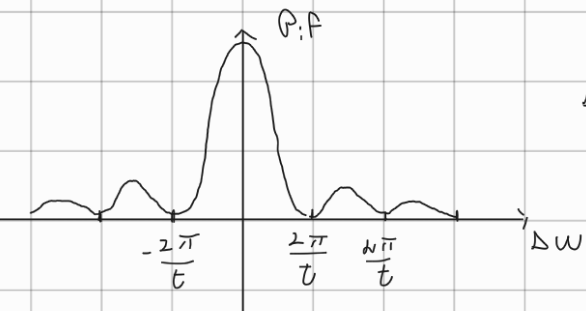
\includegraphics[width=\linewidth]{immagini/2026-05-01-14-38-09.png}
    \end{minipage}\hfill
    \begin{minipage}{0.65\textwidth}
        Se rappresentiamo $P_{if}$ in funzione di $\Delta\omega$, otteniamo la classica curva di diffrazione. %
        L'altezza del picco centrale (per $\Delta\omega \to 0$) vale: %
        \begin{equation*}
            \lim_{\Delta\omega \to 0} P_{if} = \frac{|\mathcal{L}_{fi}|^2}{\hbar^2} t^2 %
        \end{equation*}
    \end{minipage}
\end{figure}

\noindent
L'altezza cresce quadraticamente con il tempo $t$, mentre la larghezza della base del picco centrale (tra $-\frac{2\pi}{t}$ e $+\frac{2\pi}{t}$) si restringe come $1/t$. %

\noindent
Per tempi grandi ($t \to +\infty$), la funzione si restringe infinitamente diventando a tutti gli effetti proporzionale a una \textbf{Delta di Dirac}: %
\begin{equation*}
    P_{if}(\Delta\omega, t) \xrightarrow{t \to +\infty} \alpha \delta(\Delta\omega) %
\end{equation*}

\begin{figure}[H]
    \centering
    \begin{minipage}{0.3\textwidth}
        \centering
        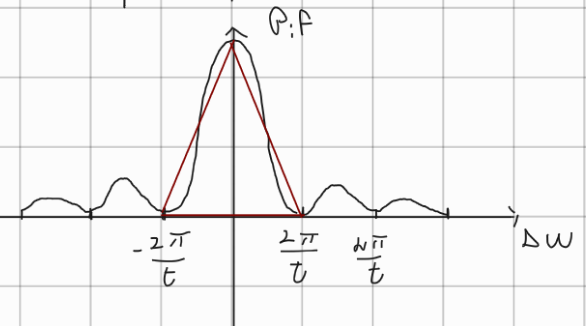
\includegraphics[width=\linewidth]{immagini/2026-05-01-14-38-50.png}
    \end{minipage}\hfill
    \begin{minipage}{0.65\textwidth}
        Calcoliamo il coefficiente di normalizzazione $\alpha$ approssimando l'area sottesa dal lobo centrale con l'area di un triangolo: %
        \begin{equation*}
            \begin{split}
                 \alpha \simeq \text{Area}_{\text{triang}} = \frac{\text{base} \times \text{altezza}}{2} = \frac{1}{2} \left( \frac{4\pi}{t} \right) \left( \frac{|\mathcal{L}_{fi}|^2 t^2}{\hbar^2} \right)\\
            = \frac{2\pi}{\hbar^2} |\mathcal{L}_{fi}|^2 t %
            \end{split}
        \end{equation*}
    \end{minipage}
\end{figure}

Quindi, per tempi lunghi, la probabilità diventa lineare nel tempo: %
\begin{equation*}
    P_{if} = \frac{2\pi}{\hbar^2} |\mathcal{L}_{fi}|^2 t \delta(\omega_f - \omega_i - \omega) \qquad \left(\text{ricordando che } \omega_f = \frac{E_f}{\hbar} , \, \omega_i = \frac{E_i}{\hbar}\right) %
\end{equation*}

\subsection{La Regola d'Oro di Fermi} %

Essendo la probabilità totale $P_{if}$ proporzionale al tempo $t$, è fisicamente molto più sensato definire il \textbf{Tasso di Transizione} (Transition Rate) $W_{if}$, ovvero la \textbf{Probabilità di transizione per unità di tempo} dividento tutto per $t$: %

\begin{equation}
    \boxed{ W_{if} = \frac{P_{if}}{t} = \frac{2\pi}{\hbar^2} |\mathcal{L}_{fi}|^2 \delta(\omega_f - \omega_i - \omega) } \quad \text{\textbf{REGOLA D'ORO DI FERMI}} %
\end{equation}

\noindent
Utilizzando la proprietà della funzione Delta $\delta(ax) = \frac{1}{a}\delta(x)$, possiamo riscrivere l'argomento in termini di energia moltiplicando per $\hbar$ e dividendo fuori: $\delta\left(\frac{E_f - E_i - \hbar\omega}{\hbar}\right) = \hbar \delta(E_f - E_i - \hbar\omega)$. La Regola d'Oro assume la sua forma più celebre: %

\begin{equation}
    \boxed{ W_{if} = \frac{2\pi}{\hbar} |\mathcal{L}_{fi}|^2 \delta(E_f - E_i - \hbar\omega) } \quad \text{(Prob. di trans. per unità di tempo)} %
\end{equation}

\noindent
\textbf{Il significato fisico fondamentale della Delta di Dirac:} %
La probabilità di transizione è strettamente nulla ($\delta = 0$) in tutti i casi, \textit{tranne} quando l'argomento della delta si annulla: %
\begin{equation*}
    E_f - E_i - \hbar\omega = 0 \quad \Rightarrow \quad \begin{cases}
        E_f = E_i + \hbar\omega \quad (\text{Assorbimento}) \\ %
        E_i = E_f - \hbar\omega \quad (\text{Emissione stimolata}) %
    \end{cases}
\end{equation*}
\begin{figure}[H]
    \centering
    \begin{minipage}{0.3\textwidth}
        \centering
        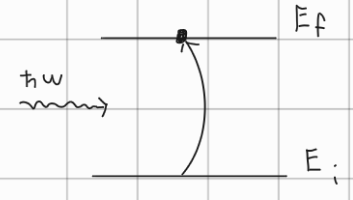
\includegraphics[width=\linewidth]{immagini/2026-05-01-14-48-24.png}
    \end{minipage}\hfill
    \begin{minipage}{0.65\textwidth}
        La matematica ha appena dimostrato naturalmente il \textbf{Principio di Conservazione dell'Energia}! Una transizione può avvenire solo ed esclusivamente se l'energia del fotone incidente ($\hbar\omega$) corrisponde esattamente al salto energetico tra i due livelli. %
    \end{minipage}
\end{figure}

\section{Assorbimento ed Emissione Stimolata} %

Ripartiamo dall'Hamiltoniana completa $\hat{H} = \hat{H}_0 + \hat{H}'$ per l'atomo di idrogeno interagente con un campo EM: %
\begin{equation*}
    \hat{H}_0 = \frac{\hat{p}^2}{2m} + \left( -\frac{e^2}{4\pi\varepsilon_0 r} \right) \quad , \quad \hat{H}' = \hat{\mathcal{L}} e^{-i\omega t} \quad \text{con } \hat{\mathcal{L}} = -\frac{e}{m} A_0 e^{i\vec{q}\cdot\vec{r}} \hat{\varepsilon} \cdot \hat{p} %
\end{equation*}
\begin{equation*}
    \Psi(\vec{r}, t) = \sum_k c_k(t) u_k(\vec{r}) e^{-i\omega_k t} \quad , \quad W_{if} = \frac{2\pi}{\hbar} |\mathcal{L}_{fi}|^2 \delta(E_f - E_i - \hbar\omega) %
\end{equation*}

\noindent
Un campo elettromagnetico reale (come un'onda piana cosinusoidale) è descritto da un potenziale vettore $\vec{A}$ che contiene \textbf{entrambe} le componenti di frequenza (positiva e negativa): %
\begin{equation}
    \vec{A}(\vec{r}, t) = A_0 \hat{\varepsilon} \left[ e^{i(\vec{q}\cdot\vec{r} - \omega t)} + e^{-i(\vec{q}\cdot\vec{r} - \omega t)} \right] %
\end{equation}

\noindent
Sostituendo questa forma completa nell'espressione dell'Hamiltoniana perturbativa $\hat{H}' = -\frac{e}{m}\vec{A}\cdot\hat{p}$, otteniamo due termini distinti: %
\begin{align*}
    \Rightarrow \hat{H}' &= -\frac{e}{m} A_0 \hat{\varepsilon} \left[ e^{i(\vec{q}\cdot\vec{r} - \omega t)} + e^{-i(\vec{q}\cdot\vec{r} - \omega t)} \right] \cdot \hat{p} = \\ %
    &= \underbrace{ \left(-\frac{e}{m}\right) A_0 e^{i\vec{q}\cdot\vec{r}} \hat{\varepsilon} \cdot \hat{p} }_{\hat{\mathcal{L}}} e^{-i\omega t} + \underbrace{ \left(-\frac{e}{m}\right) A_0 e^{-i\vec{q}\cdot\vec{r}} \hat{\varepsilon} \cdot \hat{p} }_{\hat{\mathcal{L}}^+} e^{i\omega t} %
\end{align*}

$\Rightarrow$ Rispetto ai passaggi fatti in precedenza per arrivare alla Regola d'Oro, \textbf{abbiamo un termine in più} (l'operatore aggiunto $\hat{\mathcal{L}}^+$). %
Ripercorrendo la stessa dimostrazione per le probabilità di transizione, arriviamo ad una \textbf{formulazione più completa della Regola d'Oro di Fermi}: %

\begin{equation}
    \Rightarrow \quad W_{if} = \frac{2\pi}{\hbar} \left[ |\mathcal{L}_{fi}|^2 \delta(E_f - E_i - \hbar\omega) + |\mathcal{L}_{fi}^+|^2 \delta(E_f - E_i + \hbar\omega) \right] %
\end{equation}

\noindent
Questa formula descrive due processi fisici opposti: %
\begin{enumerate}
    \item \begin{figure}[H]
        \centering
        \begin{minipage}{0.3\textwidth}
            \centering
            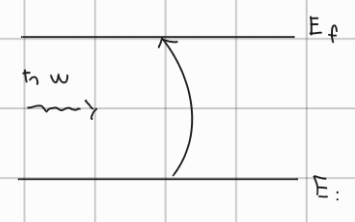
\includegraphics[width=\linewidth]{immagini/2026-05-01-14-50-33.png}
        \end{minipage}\hfill
        \begin{minipage}{0.65\textwidth}
            \textbf{ASSORBIMENTO:} Guidato dalla prima delta $\delta(E_f - E_i - \hbar\omega)$. Avviene quando \textbf{$E_f = E_i + \hbar\omega$}. L'elettrone assorbe il fotone e salta a un livello superiore. %
        \end{minipage}
    \end{figure}
    \item \begin{figure}[H]
        \centering
        \begin{minipage}{0.3\textwidth}
            \centering
            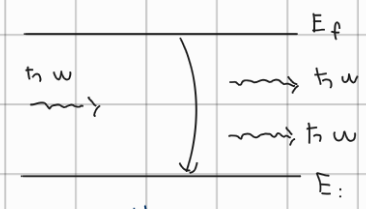
\includegraphics[width=\linewidth]{immagini/2026-05-01-14-50-48.png}
        \end{minipage}\hfill
        \begin{minipage}{0.65\textwidth}
            \textbf{EMISSIONE STIMOLATA:} Guidata dalla seconda delta $\delta(E_f - E_i + \hbar\omega)$. Avviene quando \textbf{$E_f = E_i - \hbar\omega$}. L'onda incidente "stimola" l'elettrone a decadere a un livello inferiore, emettendo un nuovo fotone in fase con l'onda incidente. %
        \end{minipage}
    \end{figure}
\end{enumerate}

\noindent
\textit{Nota cruciale: Questa NON È l'emissione spontanea (ovvero l'elettrone che decade da solo senza un campo esterno), la quale non è prevista da questo modello semiclassico!} %

\subsection{Modello Drude-Lorentz vs Meccanica Quantistica} %

Possiamo ora mettere in parallelo il modello classico della materia (dove gli elettroni sono visti come massette attaccate a molle) e i risultati esatti appena ottenuti dalla Meccanica Quantistica: %

\begin{table}[htbp]
\centering
\resizebox{\textwidth}{!}{
\begin{tabular}{|l|c|c|}
\hline
\textbf{Concetto Fisico} & \textbf{Modello Drude-Lorentz (Classico)} & \textbf{Meccanica Quantistica} \\ %
\hline
1) L'elettrone ($e^-$) è... & Un \textbf{Oscillatore Armonico} & Una \textbf{Funzione d'onda} espansa in stati \\ %
\hline
2) Frequenza di risonanza & $\omega_k$ (Frequenza propria dell'oscillatore) & Corrisponde al salto: $\hbar\omega \propto E_f - E_i$ \\ %
\hline
3) Profilo di Assorbimento & Curva a campana larga (Indice di Rifraz.) & Funzione \textbf{Delta di Dirac} $\delta(E_f - E_i - \hbar\omega)$ \\ %
\hline
4) "Forza" della transizione & $f_k$ (Oscillator Strength classico) & Elemento di matrice \textbf{$|\mathcal{L}_{fi}|^2$} \\ %
\hline
\end{tabular}}
\end{table}

\noindent
\textbf{Conclusione:} Abbiamo giustificato e derivato rigorosamente con la teoria quantistica il modello fenomenologico classico degli oscillatori di Lorentz! %

\subsection{Il Limite della Delta e l'Emissione Spontanea} %

Rimane un problema fisico di fondo. Essendo presente una Delta di Dirac ($\delta$) nella formula del tasso di transizione $W$, il salto avverrebbe \textbf{SOLO SE} l'energia del fotone $\hbar\omega$ è \textit{esattamente} uguale al salto energetico. %

\noindent
Tuttavia, la Delta perfetta si ottiene solo per un tempo di integrazione infinito ($t \to \infty$). Questo implicherebbe che l'incertezza sull'energia sia nulla ($\Delta E \to 0 \Rightarrow \Delta t \to \infty$), il che significherebbe che tutti gli stati sono perfettamente \textbf{stazionari} (vita infinita). %

\noindent
Nella realtà sperimentale, i picchi di assorbimento/emissione non sono linee infinitamente sottili ($\delta$), ma presentano un \textbf{Allargamento Naturale} (curva a campana). %
\begin{equation*}
    W_{if\ I} \simeq 10^{-2} \div 10^{-3} \quad , \quad W_{if\ II} \simeq 10^{-4} \div 10^{-6} \qquad \text{(I tassi reali sono distribuzioni, } \neq \delta) %
\end{equation*}

\noindent
\begin{figure}[H]
    \centering
    \begin{minipage}{0.3\textwidth}
        \centering
        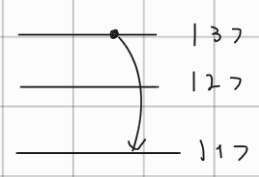
\includegraphics[width=\linewidth]{immagini/2026-05-01-14-58-05.png}
    \end{minipage}\hfill
    \begin{minipage}{0.65\textwidth}
        \textbf{Emissione Spontanea e Heisemberg:} %
        Consideriamo un elettrone in un livello eccitato. Sappiamo che, prima o poi, decade verso il basso. 
        Poiché ha un tempo di vita medio finito ($\Delta t$), per il Principio di Indeterminazione di Heisenberg avremo inevitabilmente un'incertezza sull'energia: %
    \end{minipage}
\end{figure}
\begin{equation*}
    \Delta E \Delta t \ge \frac{\hbar}{2} \quad \Rightarrow \quad \text{avendo un } \Delta t \text{ finito, abbiamo un } \Delta E \text{ non nullo!} %
\end{equation*}
Quindi l'energia del livello finale $E_f$ \textbf{non è un singolo valore esatto}, ma un piccolo range (banda). %

\noindent
Per spiegare compiutamente l'emissione spontanea (e l'allargamento naturale delle righe), non basta trattare l'atomo quantisticamente e il campo EM classicamente come abbiamo fatto finora. È necessario passare alla \textbf{Teoria dell'Elettrodinamica Quantistica (QED)}, introducendo i \textbf{Campi Quantizzati} (fotoni come quanti del campo). %

\section{Elemento di Matrice e Regola di Selezione} %

Riprendo l'elemento di matrice $\mathcal{L}_{fi}$ che compare nella Regola d'Oro di Fermi: %
\begin{equation}
    \mathcal{L}_{fi} = \int_{\mathbb{R}^3} u_f^* \hat{\mathcal{L}} u_i \, d\vec{r} \qquad , \qquad \hat{\mathcal{L}} = -\frac{e}{m} A_0 e^{i\vec{q}\cdot\vec{r}} \hat{\varepsilon} \cdot \hat{\vec{p}} %
\end{equation}

\noindent
Analizziamo il termine esponenziale spaziale dell'onda EM. Sapendo che per la luce visibile il vettore d'onda $q = \frac{2\pi}{\lambda} \simeq 10^7 \text{ m}^{-1}$ e le dimensioni atomiche sono dell'ordine di $r \simeq 1 \text{ \AA} = 10^{-10} \text{ m}$, il prodotto scalare $\vec{q}\cdot\vec{r}$ è molto piccolo ($\simeq 10^{-3}$) %.
Sviluppiamo in serie di Taylor l'esponenziale: %
\begin{equation*}
    e^{i\vec{q}\cdot\vec{r}} = 1 + \cancel{(i\vec{q}\cdot\vec{r})} + \cancel{\frac{1}{2!} (i\vec{q}\cdot\vec{r})^2} \dots %
\end{equation*}
\textbf{APPROSSIMAZIONE DI DIPOLO:} Supponendo $\vec{q}\cdot\vec{r}$ piccolo, tronchiamo lo sviluppo al primo ordine ponendo $e^{i\vec{q}\cdot\vec{r}} \simeq 1$ %.

L'elemento di matrice si semplifica: %
\begin{equation}
    \Rightarrow \quad \mathcal{L}_{fi} = -\frac{e}{m} A_0 \int u_f^* (\hat{\varepsilon} \cdot \hat{\vec{p}}) u_i \, d\vec{r} \qquad \text{con } \hat{\varepsilon} \cdot \hat{\vec{p}} = \varepsilon_x \hat{p}_x + \varepsilon_y \hat{p}_y + \varepsilon_z \hat{p}_z %
\end{equation}

\noindent
Esplicitando i prodotti scalari, possiamo studiare una singola componente, ad esempio lungo $x$: %
\begin{equation*}
    \mathcal{L}_{fi} = -\frac{e}{m} A_0 \left[ \varepsilon_x \int_{\mathbb{R}^3} u_f^* \hat{p}_x u_i \, d\vec{r} + \varepsilon_y \int_{\mathbb{R}^3} u_f^* \hat{p}_y u_i \, d\vec{r} + \varepsilon_z \int_{\mathbb{R}^3} u_f^* \hat{p}_z u_i \, d\vec{r} \right] %
\end{equation*}

Per risolvere l'integrale $\int u_f^* \hat{p}_x u_i \, d\vec{r}$, sfruttiamo una furba identità sui commutatori %. Sappiamo che $[\hat{x}, \hat{H}_0] = i\hbar \frac{\hat{p}_x}{m}$, da cui ricaviamo: %
\begin{equation*}
    \hat{p}_x = \frac{m}{i\hbar} [\hat{x}, \hat{H}_0] = \frac{m}{i\hbar} (\hat{x}\hat{H}_0 - \hat{H}_0\hat{x}) %
\end{equation*}

\noindent
Sostituendo questa identità nell'integrale e sfruttando il fatto che $\hat{H}_0$ è un operatore \textbf{Ermitiano} ($\hat{H}_0 u_i = E_i u_i$ e $u_f^* \hat{H}_0 = E_f u_f^*$) %:
\begin{align*}
    \Rightarrow \quad & \frac{m}{i\hbar} \int_{\mathbb{R}^3} u_f^* [\hat{x}, \hat{H}_0] u_i \, d\vec{r} = \frac{m}{i\hbar} \left[ \int u_f^* \hat{x} \hat{H}_0 u_i \, d\vec{r} - \int u_f^* \hat{H}_0 \hat{x} u_i \, d\vec{r} \right] = \\ %
    &= -\frac{im}{\hbar} \left[ E_i \int u_f^* \hat{x} u_i \, d\vec{r} - E_f \int u_f^* \hat{x} u_i \, d\vec{r} \right] = \frac{im}{\hbar} \underbrace{(E_f - E_i)}_{\hbar\omega_f - \hbar\omega_i} \int u_f^* \hat{x} u_i \, d\vec{r} = \\ %
    &= im\omega \int_{\mathbb{R}^3} u_f^* \hat{x} u_i \, d\vec{r} %
\end{align*}

\noindent
Riassemblando tutte le componenti spaziali, l'elemento di matrice originario diventa: %
\begin{equation*}
    \Rightarrow \quad -\frac{e}{m} A_0 (im\omega) \left[ \varepsilon_x \int u_f^* \hat{x} u_i \, d\vec{r} + \varepsilon_y \int u_f^* \hat{y} u_i \, d\vec{r} + \varepsilon_z \int u_f^* \hat{z} u_i \, d\vec{r} \right] = -i e A_0 \omega \int_{\mathbb{R}^3} u_f^* \hat{\varepsilon} \cdot \hat{\vec{r}} u_i \, d\vec{r} %
\end{equation*}

\noindent
Dal potenziale vettore ricaviamo il campo elettrico: $\vec{E} = -\frac{\partial \vec{A}}{\partial t} = i\omega A_0 \hat{\varepsilon} e^{i(\vec{q}\cdot\vec{r} - \omega t)}$. Valutando l'ampiezza complessa come $\mathcal{E}_0 = i\omega A_0 \hat{\varepsilon}$ %:
\begin{equation}
    \Rightarrow \quad \boxed{ \mathcal{L}_{fi} = -\mathcal{E}_0 \int_{\mathbb{R}^3} u_f^* \underbrace{ (e\hat{\vec{r}}) }_{\text{Momento di Dipolo } \Rightarrow e\hat{\vec{r}} = \hat{\vec{d}}} u_i \, d\vec{r} } %
\end{equation}

L'Hamiltoniana di interazione si semplifica elegantemente a: %
\begin{equation}
    \hat{H}_{int} = \hat{\mathcal{L}} e^{-i\omega t} = -\mathcal{E}_0 \cdot \hat{\vec{d}} e^{-i\omega t} = -\vec{E} \cdot \hat{\vec{d}} \qquad \text{(Interazione classica tra campo E e dipolo)} %
\end{equation}

\noindent
Perché vi sia una probabilità di transizione non nulla (Regola d'Oro), l'\textbf{elemento di matrice del raggio} $\vec{r}_{fi}$ non deve annullarsi: %
\begin{equation}
    \vec{r}_{fi} = \int_{\mathbb{R}^3} u_f^* \hat{\vec{r}} u_i \, d\vec{r} \neq 0 %
\end{equation}

\noindent
Le funzioni d'onda atomiche $u_k = R_{nl}(r)Y_l^m(\theta,\varphi)$ hanno una \textbf{parità} ben definita, determinata interamente dal numero quantico orbitale $l$ tramite le armoniche sferiche %:
\begin{equation*}
    Y_l^m(\pi - \theta, \varphi + \pi) = (-1)^l Y_l^m(\theta, \varphi) %
\end{equation*}
\textbf{LA PARITÀ È DATA DA $\mathbf{l}$.} %

\noindent
Valutiamo l'integrale $\vec{r}_{fi} = \int u_f^* \hat{\vec{r}} u_i \, d\vec{r}$. Sappiamo che l'operatore posizione $\hat{\vec{r}}$ è \textbf{dispari} %.
Affinché l'integrale su tutto lo spazio di una funzione (il prodotto $u_f^* \hat{\vec{r}} u_i$) non sia identicamente zero, la funzione integranda totale deve essere \textbf{pari}. Poiché $\hat{\vec{r}}$ è dispari, è necessario che $u_f$ e $u_i$ abbiano \textbf{parità opposta}! %
\begin{equation*}
    \Rightarrow \text{Perché } r_{fi} \text{ non sia nullo, } u_f \text{ e } u_i \text{ \textbf{non possono avere la stessa PARITÀ}}. %
\end{equation*}

\noindent
Questo implica che in una transizione di dipolo, il salto del numero quantico orbitale $\Delta l = l_f - l_i$ deve essere un numero dispari ($\pm 1, \pm 3, \pm 5 \dots$). Un'analisi matematica più rigorosa (che omettiamo) restringe ulteriormente questa condizione a: %
\begin{equation}
    \boxed{ \Delta l = \pm 1 } \quad \Rightarrow \quad \text{\textbf{REGOLA DI SELEZIONE DI DIPOLO ELETTRICO}} %
\end{equation}\\

\noindent
\textbf{Esempio Pratico:} %
Consideriamo l'assorbimento di un fotone da parte di un elettrone nello stato fondamentale $1s$ ($n=1, l=0$). %
\begin{figure}[H]
    \centering
    \begin{minipage}{0.3\textwidth}
        \centering
        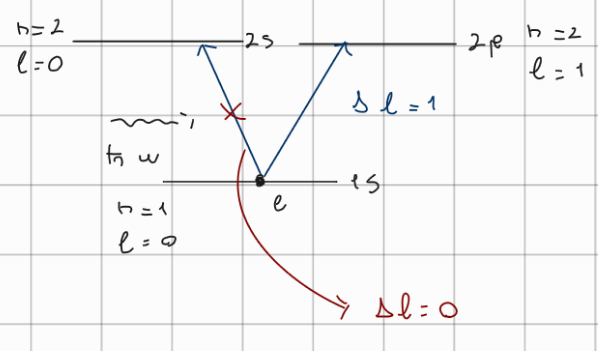
\includegraphics[width=\linewidth]{immagini/2026-05-01-15-03-46.png}
    \end{minipage}\hfill
    \begin{minipage}{0.65\textwidth}
        \begin{itemize}
            \item Transizione $1s \to 2p$ ($n=2, l=1$): È permessa perché $\Delta l = +1$. %
            \item Transizione $1s \to 2s$ ($n=2, l=0$): È \textbf{proibita} per l'assorbimento di un fotone (in approssimazione di dipolo) perché $\Delta l = 0$. %
        \end{itemize}
    \end{minipage}
\end{figure}

\noindent
Cosa succede allo stato $2s$ (che non può diseccitarsi verso il basso emettendo un fotone di dipolo)? Diventa uno \textbf{STATO METASTABILE} (con vita media molto lunga, $\Delta t \simeq 0.1 \text{ s}$). %

\noindent
\textit{Nota finale:} Come decade allora? Rivedendo lo sviluppo di Taylor iniziale dell'esponenziale $e^{i\vec{q}\cdot\vec{r}} = 1 + i\vec{q}\cdot\vec{r} + \frac{1}{2}(i\vec{q}\cdot\vec{r})^2 \dots$, notiamo che se l'approssimazione di dipolo (il termine $1$) dà risultato nullo, \textbf{esistono comunque gli altri termini}! %
Questi termini successivi danno origine a transizioni più deboli chiamate di \textbf{Dipolo Magnetico} o \textbf{Quadrupolo Elettrico}, che seguono regole di selezione differenti e permettono al sistema di decadere comunque, seppur molto più lentamente. %

% --- FINE BLOCCO ---




\end{document}